%!TEX root = ../main.tex
\section{Benchmark Design} 
In this section, we first introduce the design goals of \sys benchmark for table discovery tasks, and then present how to generate the \sys benchmark consisting of datasets, queries and ground truth.

\subsection{Design Goals}
We design the table discovery benchmark by the 
benchmark design criteria proposed by Jim Gray.

\noindent\textbf{Relevance.}
The benchmark covers a wide range of table discovery characteristics. First, in terms of the data lake, we incorporate 4 lakes with size ranging from 10GB to 1TB, and with column number ranging from \cc{1 million} to 10 million. Second, in terms of the queries, with the help of much human efforts, we create and label more than 10 thousand table queries that cover various query characteristics, including column semantic, column overlapping, column size, etc.



\noindent\textbf{Scalability.} The benchmark involves much larger data lakes than existing data lakes for table discovery. The data lake size should be considered from two aspects. One is the normal total storage size that is highly related  to the average table size  and the number of tables. The other is the number of total columns because almost all table discovery algorithms build index and search over a large number of columns.  \sys involves up to 1 TB data lake and 10 million columns, which is sufficient enough to evaluate the scalability.




\noindent\textbf{Simplicity.} The benchmark designs easy-to-use APIs to support table discovery in data lakes. Users can simply leverage few lines of codes to query our benchmark datasets using different algorithms and compare with them.
\cc{seems limited}





\begin{figure}[h]
	\centering
	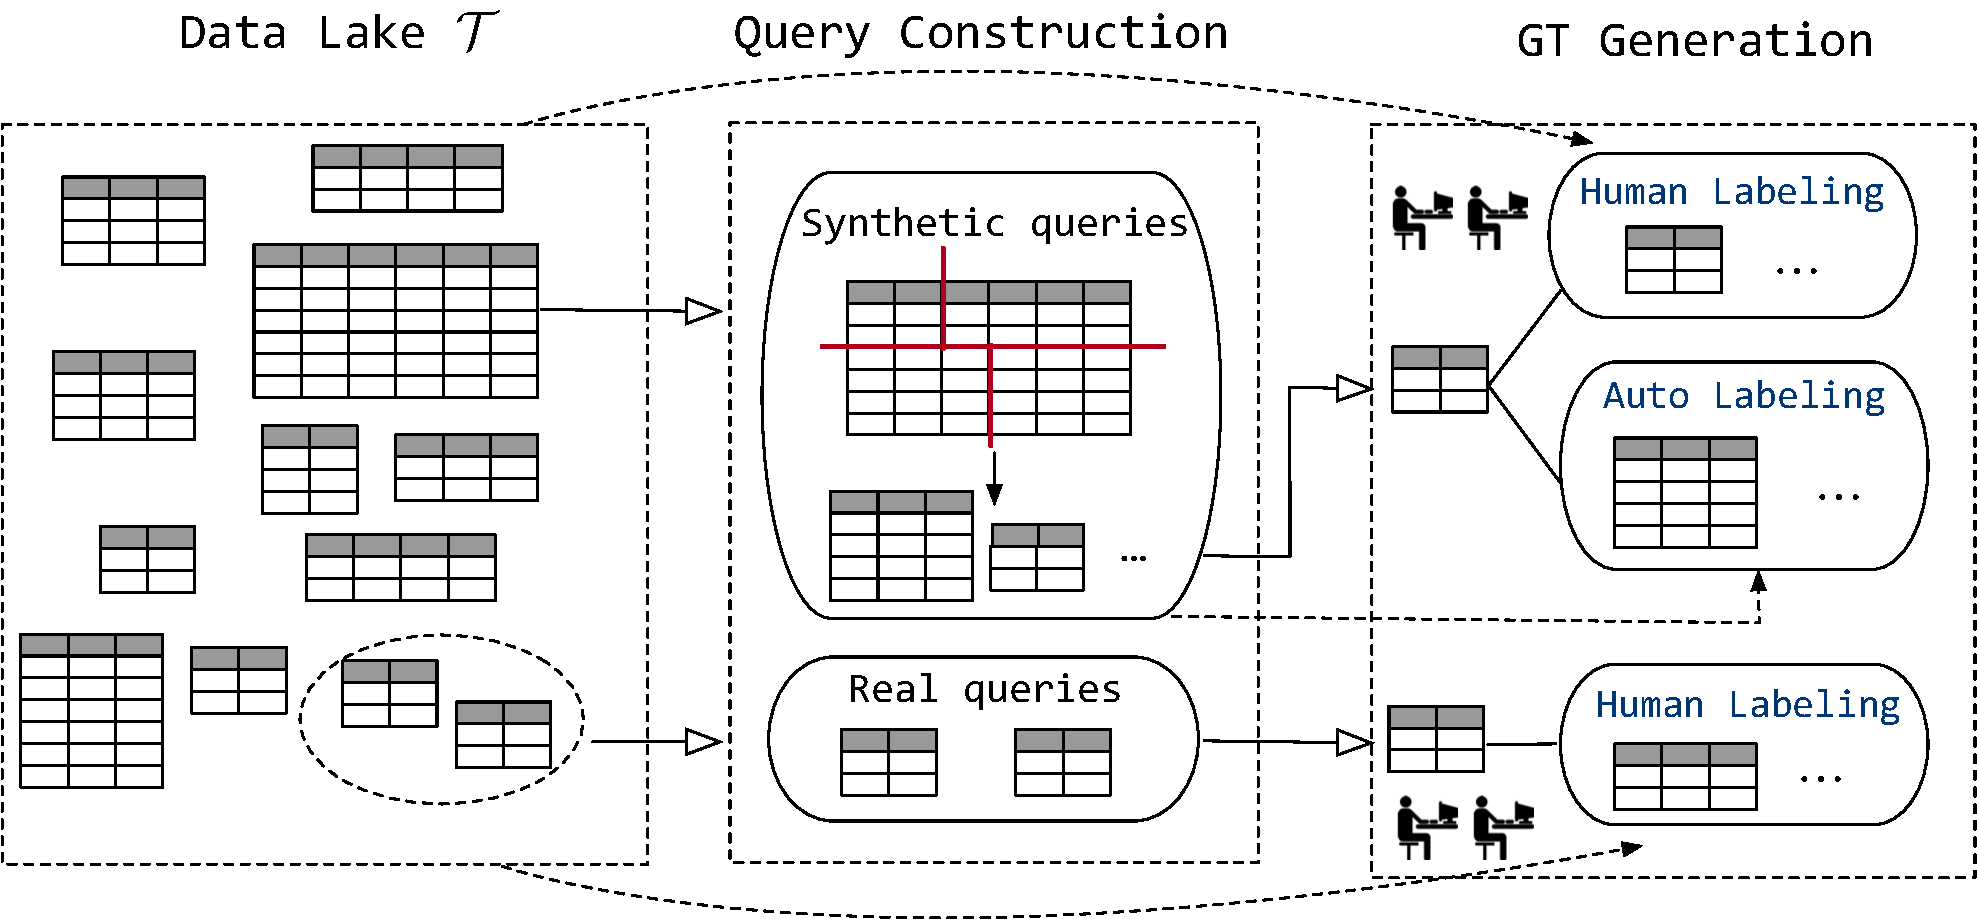
\includegraphics[width=1\linewidth]{fig/benchmark.pdf}
	\caption{Overview of \sys Construction.}
	\label{fig:benchmark}
\end{figure}



\subsection{Benchmark Overview}
In this subsection, we overview the pipeline of our benchmark design. Overall, as shown in Figure~\ref{fig:benchmark}, we first collect the datasets, then construct queries and generate ground truth for these queries. Finally, we implement various table discovery algorithms, analyze their performance from multiple perspectives, and design easy-to-use APIs.


\begin{table*}[t]
	\centering
	\caption{Statistics of Data Lakes.}
	\begin{tabular}{|c|c|c|c|c|c|}
		\hline
		\centering
		Data Lake  & \#-Tables & $\#$-Columns & Max/Min/Avg Col. No. & Max/Min/Avg Row No. & Size (GB)  \\
		\hline  
		OpenData Small& 10,374  & 166,770 & 502/3/16.1  &  10,250,220/5/79,310.7  & 100.03GB  \\
		\hline
		OpenData Large& 64,793  & 1,385,149  & 502/3/21.0   & 39,014,091/5/112,359.9  & 1.08TB   \\
		\hline
		WebTable Small& 2,772,825   & 17,929,497 & 25/3/6.5  & 16,908/5/23.0  &13.01GB \\
		\hline
		WebTable Large& 16,684,293  & 107,891,225 & 25/3/6.8  & 16,908/5/23.5   & 77.05G  \\
		\hline
	\end{tabular}
	\label{Table:datasets}
	
\end{table*}

\noindent\textbf{Datasets.}
We build 4 data lakes from OpenData~\cite{OpenData} and WebTable~\cite{WebTable}. For each data source, we create a small and large data lake respectively. The statistics of them are shown in Table~\ref{Table:datasets}.
For OpenData~\cite{OpenData}, we extract 70,546 tables from \cc{XXX}, including the union of \cc{XX}, \cc{XX} and \cc{XX}. The characteristic of OpenData is that it contains large tables with numerous rows. 
For WebTable~\cite{WebTable}, the original dataset contains 27,783,441 tables, from which we extract 50\% into the data lake. The characteristic of WebTable is that it contains a large number of small tables, and thus the total number of columns is very large. As a pre-processing, we remove some very small tables (row number $<5$ or column number $<3$) and remove the columns with larger then 50\% NULL values. Finally, we obtain the OpenData Large and WebTable Large, from which we randomly sample 10\% as OpenData Small and WebTable Small, as shown in Table~\ref{Table:datasets}.

%after adding the small tables or before ??

%Table~\ref{table} summarizes the statistics of collected datasets.


\noindent\textbf{Query Construction.} We use two methods to construct join \& union search queries.

\noindent \underline{\textit{Real queries.}}  A direct way  is to use real tables  as queries, so we  extract  $Q\subset \lake$ as a set of queries. However, in real scenarios, the table search results are likely to be sparse, so in all previous benchmarks, they construct synthetic queries based on big tables, and we conduct this in a similar way as follows.

\noindent \underline{\textit{Synthetic queries.}} The basic idea is to split large tables into multiple small ones. As shown in Figure~\ref{fig:benchmark}, generally, we split from two perspectives, namely row-level and column-level splitting. 
Basically, row-level splitting mainly generates unionable tables, while column-level splitting mostly generates joinable tables.
These small tables are then put into the data lake and they can also serve as queries.
%Split large tables into small ones, which are put into the data lake, and then use some of the small ones as queries.  

\noindent\textbf{Ground Truth Generation.} For different query construction methods, the ways of ground truth (GT) generation are different, as shown in Figure~\ref{fig:benchmark}.

 \noindent \underline{\textit{GT generation for real queries.}} An ideal ground truth generation method is that for each of queries, we ask the humans to label whether all tables in $\lake$ can be join/union with the query, which is prohibitively expensive. A natural solution is to leverage a rough search  method to retrieve a number of candidate tables that have a relatively high relevance with the query table, \ie a high recall, and then ask the humans to manually check these candidates.
 
 \noindent \underline{\textit{GT generation for synthetic queries.}} We can see from  Figure~\ref{fig:benchmark} that the ground truth of synthetic queries consists of two parts. 
 On the one hand, since each synthetic query is obtained by splitting from a big table, there exist multiple tables splitted from the same table that are joinable/unionable with the query. 
  On the other hand, very likely, there  still exist joinable/unionable tables in $\lake$ besides the above  splitted ones.  Therefore, we leverage the above method for  real queries to label more ground truth via humans.




\iffalse
+ Classify: 

\quad\quad -- Column type (string, number, category)
 
\quad\quad -- Fake or real
  
\quad\quad -- Selectivity

\quad\quad -- Size

\noindent\textbf{Ground Truth Creation.}
\fi


\noindent\textbf{Method Evaluation \& Analysis.} 
Given the data lakes, queries and ground truth, we next compare the performance of different table discovery approaches about the effectiveness and efficiency. Overall, in terms of the downstream task, we categorize existing methods based on supporting join, union or join\&union search. In each category, different methods adopt different column representation and index construction methods, which also lead to different online query methods, with different performance on effectiveness and efficiency. Furthermore, \cc{how to summarize the query categories???}
%but they can support each other by slightly modifying. To support our query-candidate category, we have to apply Starmie (for union) to the join scenario.

+ Query Category: Real/Synthetic (Sparse/Dense), String/Category/Numerical (Distinguish)

+ Query-Candidate Category: Join(overlap, semantic), Union(overlap, semantic)


\iffalse
\cc{How to category}

+ \cc{Join/Union}

+ \cc{Schema matching}

+ Hash-based

+ Inverted index 

+ Pre-trained language model (HNSW)


\fi


\noindent\textbf{API Design.}

    \begin{table*}[t]
        \centering
        \caption{Table Discovery Methods.}
        \begin{tabular}{|c|c|c|c|cccc|}
            \hline
            \multirow{2}{1cm}{\textbf{Methods}} & \multirow{2}{0.6cm}{\textbf{Task}} & \multirow{2}{0.8cm}{\textbf{Index}} & \multirow{2}{1.6cm}{\textbf{Embedding}} & \multicolumn{2}{c}{\textbf{Offline Process}} & \multicolumn{2}{c|}{\textbf{Online Process}} \\
            &&&&Time Comp.    & Space Comp. & Time Comp. & Space Comp. \\ 
            \hline
            \josie~\cite{Josie} & J & Inv. index & \XSolidBrush  & O$(\cellvaluenum + \rawtokennum \log \rawtokennum)$         & O$(\rawtokennum)$                   & O$(\positinglistlen log \positinglistlen)$         & O$(\positinglistlen)$    \\
            \hline
            \lsh~\cite{LshEn} & J & LSH & \XSolidBrush& O$(\columnnum)$        & O$(\columnnum \times \minhashlen)$                   & O$(\querycolumnnum)$                & O$(\querycolumnnum \times \minhashlen)$  \\
            \hline
            \pex~\cite{Pexeso} & J &  Inv. index& \Checkmark  & O$(\rawtokennum)$        & O$(\rawtokennum)$                   & O$(\log \querycellvalue \times \log \rawtokennum)$                & O$(\querycellvalue)$     \\
            \hline
            \deepjoin~\cite{DeepJoin} & J & HNSW & \Checkmark & O$(\columnnum)$         & O$(\columnnum)$                   & O$(\log \columnnum)$                & O$(\columnnum)$  \\
            \hline
             \tus~\cite{TUS} & U & LSH & \Checkmark  & O$(\cellvaluenum + \columnnum)$         & O$(\columnnum \times \minhashlen)$    & O$(\querycolumnnum)$               &  O$(\querycolumnnum \times \minhashlen)$     \\
            \hline
            \dlll~\cite{D3L} & U & LSH & \Checkmark& O$(\cellvaluenum + \columnnum)$          & O$(\columnnum)$                   & O$(\querycolumnnum \times \dlllneighbornnum)$                & O($\querycolumnnum$)      \\
            \hline
            \starmie~\cite{Starmie} & U & HNSW & \Checkmark & O$(\columnnum)$         & O$(\columnnum)$                   & O$(\log \columnnum)$                & O$(\columnnum)$   \\
            \hline
            \santos~\cite{Santos} & U & Inv. index & \XSolidBrush & O$(\rawtokennum)$         & O$(\rawtokennum \times \columnnum {\averagetargetcolumnnum}^2)$    & O$(\querycellvalue + \santosneighbornnum)$               & O$(\querycellvalue)$  \\
            \hline
            \frt~\cite{Frt12} & J \& U & N/A & \XSolidBrush &  O$(\columnnum)$        & O$(\columnnum)$    & O$( \tablenum \times {(\querycolumnnum + \averagetargettuplenum)}^3)$               & O$({\averagetargettuplenum}^2)$    \\
            \hline
            \infogather~\cite{InfoGather} & J \& U & Inv. index & \XSolidBrush & O$(\columnnum^2)$   & O$(\columnnum^2)$    & O$(\querycolumnnum \times \inforneighbornnum \log \inforneighbornnum)$              & O$(\inforneighbornnum )$   \\
            \hline
            \aurum~\cite{Aurum} & J \& U & LSH & \Checkmark  & O$(\columnnum)$         & O$(\columnnum)$                   & O$(\log \columnnum)$                & O$(\columnnum)$   \\
            \hline
            Pretrain-based~\cite{} & U & HNSW & \Checkmark   & O$(\columnnum)$         & O$(\columnnum)$                   & O$(\log \columnnum)$                & O$(\columnnum)$ \\
            \hline
        \end{tabular}
        \label{table:methods}
        
    \end{table*}

\begin{table}[!ht]
	\centering
	\caption{The Meaning of Different Symbols.}
	\begin{tabular}{cc}
		\hline
		Symbol & Meaning \\ \hline
		$\mathcal{B}$ & \#-Columns in the query table $\qtable$  \\
		$\mathcal{N}$ &\#-Columns in all tables $\lake$ \\
		$\mathcal{K}$ & \#-Non-distinct cell values in all tables in $\lake$   \\
		$\mathcal{R}$ &\#-Distinct cell values in all tables in $\lake$ \\
		$\mid \mathcal{T} \mid$ & \#-Tables in $\lake$  \\
		$\mathcal{X}$ &\#-Tuples in all tables in $\lake$ \\
		$\mathcal{A}$ & \#-Non-distinct cell values in query table $\qtable$  \\
		
		$\mathcal{L}$ & The length of positing list in \josie  \\
		$\mathcal{H}$ & The dimension of minhash vector \\
		$\mathcal{P}$ & \#-Partitions in \lsh\\
		$\mathcal{D}$ & \#-Neighbors in \dlll\\
		$\mathcal{I}$ & \#-Neighbors in \infogather\\
		$\overline{\mathcal{O}}$ & The average number of cloumns in candidate tables\\
		%


%fake方法造query:就是先选一个行和列都比较多的大表,然后随机选择num列(num为随机数),并且打乱这些列的顺序,再添加了一列随机数;竖着切成几个小表之后,再随机选择num行(num为随机数),并且打乱这些行的顺序,同时,选择横着切表之前的1/4行作为切完之后各个小表之间的overlap。

%不fake方法造query:随机抽选一些候选表出来,然后再人工抽取一些人能识别出来表格主题的表(方便后续ground truth的标注)

%fake方法定ground truth: 首先,竖着切之后,判断各个小表有没有属性重复,有的话,两个表之间视为可以join。除此之外,横着切生成的不同小表,由于它们之间一定会有overlap和属性重复,所以两两之间视为可union

%不fake方法定ground truth:根据不fake的方法造出来的query,利用一些简单的相似性判断捞出一些候选表,再进行人工标注

	
	\end{tabular}
	\label{symbol_table}
\end{table}



